\documentclass[aspectratio=169]{beamer}

% ─── Theme & Colors ───────────────────────────────────────────────────────
\usetheme{default}
\usefonttheme{professionalfonts}

\definecolor{MuncheezBlue}{RGB}{0, 102, 204}
\definecolor{MuncheezDark}{RGB}{20, 20, 20}
\definecolor{MuncheezGray}{RGB}{120, 120, 120}
\definecolor{MuncheezLight}{RGB}{245, 245, 245}

\setbeamercolor{structure}{fg=MuncheezBlue}
\setbeamercolor{background canvas}{bg=white}
\setbeamercolor{normal text}{fg=MuncheezDark}
\setbeamercolor{frametitle}{fg=white, bg=MuncheezBlue}
\setbeamercolor{title}{fg=white, bg=MuncheezBlue}
\setbeamercolor{block title}{fg=white, bg=MuncheezBlue}
\setbeamercolor{block body}{bg=MuncheezLight, fg=MuncheezDark}
\setbeamercolor{item}{fg=MuncheezBlue}
\setbeamercolor{section in toc}{fg=MuncheezBlue}
\setbeamercolor{subsection in toc}{fg=MuncheezGray}

% ─── Fonts ────────────────────────────────────────────────────────────────
\setbeamerfont{frametitle}{size=\Large, series=\bfseries}
\setbeamerfont{title}{size=\huge, series=\bfseries}
\setbeamerfont{subtitle}{size=\large, series=\mdseries}
\setbeamerfont{author}{size=\normalsize, series=\mdseries}
\setbeamerfont{date}{size=\small, series=\mdseries}
\setbeamerfont{block title}{size=\normalsize, series=\bfseries}
\setbeamerfont{block body}{size=\small, series=\mdseries}
\setbeamerfont{itemize item}{size=\small, series=\bfseries}
\setbeamerfont{itemize subitem}{size=\footnotesize, series=\mdseries}

% ─── Layout ───────────────────────────────────────────────────────────────
\setbeamersize{text margin left=24mm, text margin right=24mm}
\setbeamersize{frametitle=\baselineskip}
\setbeamertemplate{navigation symbols}{}
\setbeamertemplate{footline}[frame number]
\setbeamertemplate{headline}{}

% ─── Logo Command ─────────────────────────────────────────────────────────
\newcommand{\muncheezlogo}{%
  \textbf{\Large M}uncheez\textcolor{MuncheezBlue}{\textbf{.}}%
}

% ─── Slide Title Template ─────────────────────────────────────────────────
\setbeamertemplate{frametitle}{%
  \vspace{2mm}%
  \textbf{\large\insertframetitle}%
  \vspace{1mm}%
}

% ─── Packages ─────────────────────────────────────────────────────────────
\usepackage{tikz}
\usetikzlibrary{shapes.geometric, arrows.meta, positioning, calc, fit, backgrounds}
\usepackage{graphicx}
\usepackage{booktabs}
\usepackage{multicol}
\usepackage{fontawesome5}
\usepackage{hyperref}
\usepackage{xcolor}
\usepackage{amsmath}

% ─── Custom Commands ──────────────────────────────────────────────────────
\newcommand{\bluebullet}{\textcolor{MuncheezBlue}{\textbullet}}
\newcommand{\sectiontitle}[1]{\textbf{\large #1}}
\newcommand{\stat}[2]{\textbf{\Large #1}\\\small #2}
\newcommand{\flowarrow}{\tikz[baseline=-0.5ex]{\draw[->, thick, MuncheezBlue] (0,0) -- (0.8,0);}}

% ─── Title Page ───────────────────────────────────────────────────────────
\title{\muncheezlogo}
\subtitle{Local commerce, delivered.}
\author{Muncheez}
\date{Pre-Seed Investor Deck \textbullet\ 2025}

\begin{document}

% ═══════════════════════════════════════════════════════════════════════════
% SLIDE 1: TITLE
% ═══════════════════════════════════════════════════════════════════════════
\begin{frame}[plain]
  \centering
  \vfill
  
\begin{tikzpicture}
    \node[text width=0.9\textwidth, align=center] at (0,0) {
      {\fontsize{48}{52}\selectfont\textbf{\muncheezlogo}}\\[8mm]
      {\Large Local commerce, delivered.}\\[4mm]
      {\normalsize Pre-Seed Investor Deck \textbullet\ 2025}
    };
  \end{tikzpicture}
  \vfill
\end{frame}

% ═══════════════════════════════════════════════════════════════════════════
% SLIDE 2: THE PROBLEM
% ═══════════════════════════════════════════════════════════════════════════
\begin{frame}{The Problem}
  \begin{columns}[T]
    \begin{column}{0.48\textwidth}
      \sectiontitle{A huge part of the food economy\\is invisible online.}
      \vspace{4mm}
      
      \textbf{Home cooks. Small vendors. Neighborhood businesses. Micro-restaurants. Informal producers.}
      
      \vspace{4mm}
      
      Many are difficult to discover, order from, and access digitally.
    \end{column}
    \begin{column}{0.48\textwidth}
      \sectiontitle{At the same time...}
      \vspace{4mm}
      
      Customers increasingly want convenience and delivery.
      
      \vspace{4mm}
      
      Existing platforms organize around established restaurants already capable of operating digitally.
      
      \vspace{4mm}
      
      \textbf{\textcolor{MuncheezBlue}{The supply that is hardest to access is the supply that needs the platform most.}}
    \end{column}
  \end{columns}
\end{frame}

% ═══════════════════════════════════════════════════════════════════════════
% SLIDE 3: THE INSIGHT
% ═══════════════════════════════════════════════════════════════════════════
\begin{frame}{The Insight}
  \centering
  \vspace{6mm}
  
  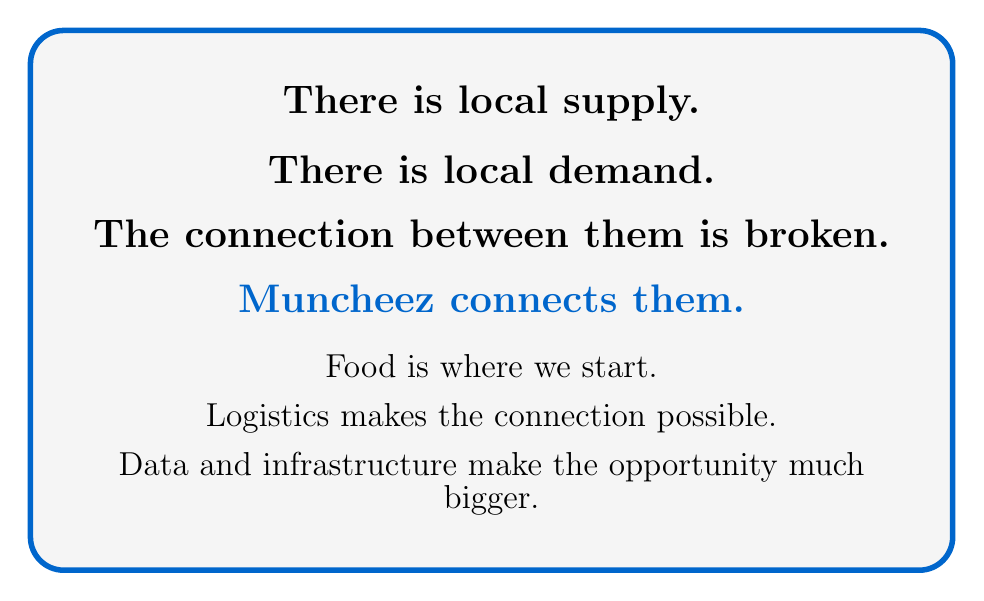
\begin{tikzpicture}
    \node[draw=MuncheezBlue, line width=2pt, rounded corners=12pt, inner sep=20pt, fill=MuncheezLight] {
      \begin{minipage}{0.85\textwidth}
        \centering
        {\Large\bfseries There is local supply.}\\[4mm]
        {\Large\bfseries There is local demand.}\\[4mm]
        {\Large\bfseries The connection between them is broken.}\\[4mm]
        {\Large\bfseries\textcolor{MuncheezBlue}{Muncheez connects them.}}\\[4mm]
        {\large Food is where we start.}\\[2mm]
        {\large Logistics makes the connection possible.}\\[2mm]
        {\large Data and infrastructure make the opportunity much bigger.}
      \end{minipage}
    };
  \end{tikzpicture}
  
  \vspace{6mm}
\end{frame}

% ═══════════════════════════════════════════════════════════════════════════
% SLIDE 4: THE SOLUTION
% ═══════════════════════════════════════════════════════════════════════════
\begin{frame}{The Solution}
  \centering
  \vspace{4mm}
  
  {\Large\bfseries LOCAL SUPPLY \flowarrow\ \muncheezlogo\ \flowarrow\ LOCAL DEMAND}
  
  \vspace{8mm}
  
  
\begin{tikzpicture}
    \node[draw=MuncheezBlue, line width=1.5pt, rounded corners=8pt, fill=white, inner sep=12pt] (discovery) {\textbf{Discovery}};
    \node[draw=MuncheezBlue, line width=1.5pt, rounded corners=8pt, fill=white, inner sep=12pt, right=1.2cm of discovery] (ordering) {\textbf{Ordering}};
    \node[draw=MuncheezBlue, line width=1.5pt, rounded corners=8pt, fill=white, inner sep=12pt, right=1.2cm of ordering] (payment) {\textbf{Payment}};
    \node[draw=MuncheezBlue, line width=1.5pt, rounded corners=8pt, fill=white, inner sep=12pt, right=1.2cm of payment] (location) {\textbf{Location}};
    \node[draw=MuncheezBlue, line width=1.5pt, rounded corners=8pt, fill=white, inner sep=12pt, right=1.2cm of location] (logistics) {\textbf{Logistics}};
    \node[draw=MuncheezBlue, line width=1.5pt, rounded corners=8pt, fill=white, inner sep=12pt, right=1.2cm of logistics] (delivery) {\textbf{Delivery}};
    
    \draw[->, thick, MuncheezBlue] (discovery) -- (ordering);
    \draw[->, thick, MuncheezBlue] (ordering) -- (payment);
    \draw[->, thick, MuncheezBlue] (payment) -- (location);
    \draw[->, thick, MuncheezBlue] (location) -- (logistics);
    \draw[->, thick, MuncheezBlue] (logistics) -- (delivery);
  \end{tikzpicture}
  
  \vspace{6mm}
  {\small\itshape Every step is designed around fragmented local supply, not established restaurants.}
\end{frame}

% ═══════════════════════════════════════════════════════════════════════════
% SLIDE 5: WHY FOOD FIRST?
% ═══════════════════════════════════════════════════════════════════════════
\begin{frame}{Why Food First?}
  \begin{columns}[T]
    \begin{column}{0.5\textwidth}
      \sectiontitle{Food creates frequent demand.}
      \vspace{4mm}
      
      People eat every day. That gives Muncheez the opportunity to:
      
      \vspace{3mm}
      \begin{itemize}
        \item Build repeated transactions
        \item Learn local demand patterns
        \item Establish a reliable logistics network
      \end{itemize}
      
      \vspace{4mm}
      Food is the \textbf{starting point}, not the final category.
    \end{column}
    \begin{column}{0.45\textwidth}
      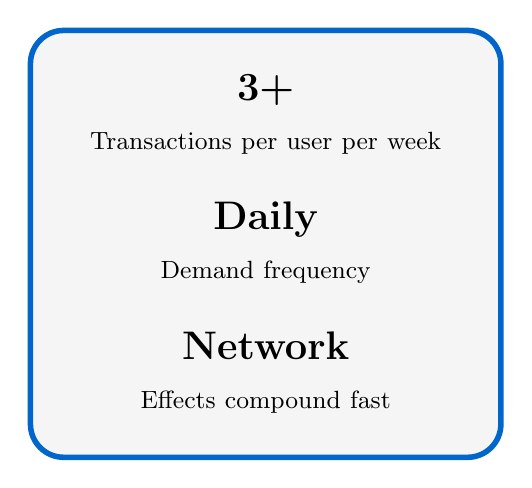
\begin{tikzpicture}
        \node[draw=MuncheezBlue, line width=2pt, rounded corners=12pt, fill=MuncheezLight, inner sep=16pt, text width=0.4\textwidth, align=center] {
          {\Large\bfseries 3+}\\[2mm]
          {\small Transactions per user per week}\\[6mm]
          {\Large\bfseries Daily}\\[2mm]
          {\small Demand frequency}\\[6mm]
          {\Large\bfseries Network}\\[2mm]
          {\small Effects compound fast}
        };
      \end{tikzpicture}
    \end{column}
  \end{columns}
\end{frame}

% ═══════════════════════════════════════════════════════════════════════════
% SLIDE 6: THE LARGER OPPORTUNITY
% ═══════════════════════════════════════════════════════════════════════════
\begin{frame}{The Larger Opportunity}
  \centering
  \vspace{4mm}
  
  
\begin{tikzpicture}
    \node[text width=0.9\textwidth, align=center] at (0,0) {
      {\Large\bfseries Once Muncheez understands:}
    };
  \end{tikzpicture}
  
  \vspace{4mm}
  
  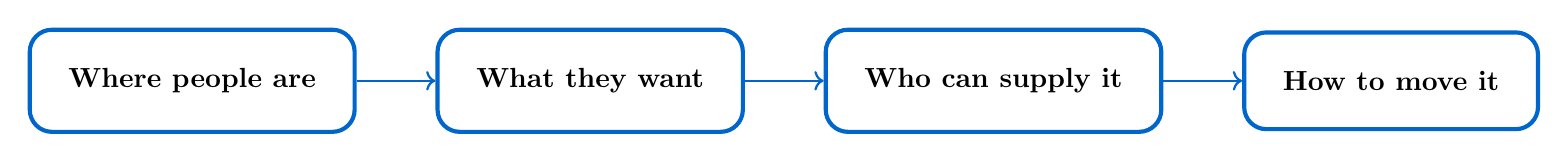
\begin{tikzpicture}
    \node[draw=MuncheezBlue, line width=1.5pt, rounded corners=8pt, fill=white, inner sep=14pt] (where) {\textbf{Where people are}};
    \node[draw=MuncheezBlue, line width=1.5pt, rounded corners=8pt, fill=white, inner sep=14pt, right=1cm of where] (what) {\textbf{What they want}};
    \node[draw=MuncheezBlue, line width=1.5pt, rounded corners=8pt, fill=white, inner sep=14pt, right=1cm of what] (who) {\textbf{Who can supply it}};
    \node[draw=MuncheezBlue, line width=1.5pt, rounded corners=8pt, fill=white, inner sep=14pt, right=1cm of who] (how) {\textbf{How to move it}};
    
    \draw[->, thick, MuncheezBlue] (where) -- (what);
    \draw[->, thick, MuncheezBlue] (what) -- (who);
    \draw[->, thick, MuncheezBlue] (who) -- (how);
  \end{tikzpicture}
  
  \vspace{6mm}
  
  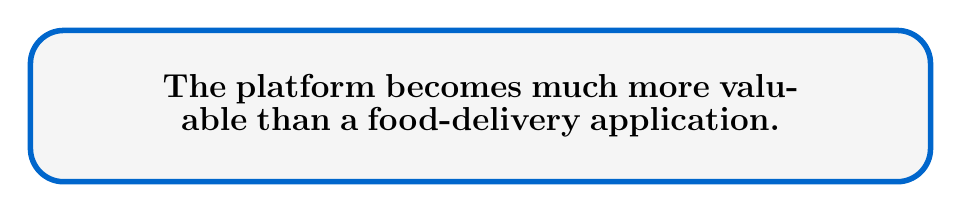
\begin{tikzpicture}
    \node[draw=MuncheezBlue, line width=2pt, rounded corners=12pt, fill=MuncheezLight, inner sep=16pt, text width=0.85\textwidth, align=center] {
      {\large\bfseries The platform becomes much more valuable than a food-delivery application.}
    };
  \end{tikzpicture}
  
  \vspace{4mm}
  {\small\itshape One long-term opportunity: practical location intelligence for neighborhoods without reliable street addresses.}
\end{frame}

% ═══════════════════════════════════════════════════════════════════════════
% SLIDE 7: LOGISTICS NETWORK
% ═══════════════════════════════════════════════════════════════════════════
\begin{frame}{Logistics Network}
  \centering
  \vspace{4mm}
  
  {\Large\bfseries The delivery method should fit the job.}
  
  \vspace{6mm}
  
  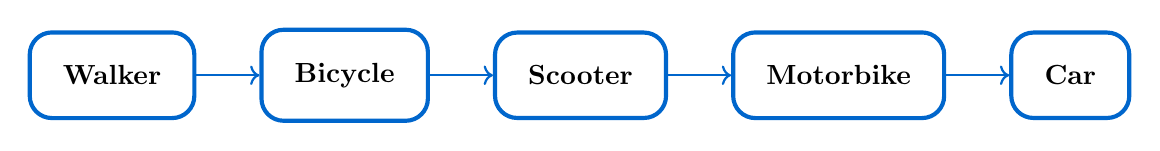
\begin{tikzpicture}
    \node[draw=MuncheezBlue, line width=1.5pt, rounded corners=8pt, fill=white, inner sep=12pt] (walk) {\textbf{Walker}};
    \node[draw=MuncheezBlue, line width=1.5pt, rounded corners=8pt, fill=white, inner sep=12pt, right=0.8cm of walk] (bike) {\textbf{Bicycle}};
    \node[draw=MuncheezBlue, line width=1.5pt, rounded corners=8pt, fill=white, inner sep=12pt, right=0.8cm of bike] (scooter) {\textbf{Scooter}};
    \node[draw=MuncheezBlue, line width=1.5pt, rounded corners=8pt, fill=white, inner sep=12pt, right=0.8cm of scooter] (moto) {\textbf{Motorbike}};
    \node[draw=MuncheezBlue, line width=1.5pt, rounded corners=8pt, fill=white, inner sep=12pt, right=0.8cm of moto] (car) {\textbf{Car}};
    
    \draw[->, thick, MuncheezBlue] (walk) -- (bike);
    \draw[->, thick, MuncheezBlue] (bike) -- (scooter);
    \draw[->, thick, MuncheezBlue] (scooter) -- (moto);
    \draw[->, thick, MuncheezBlue] (moto) -- (car);
  \end{tikzpicture}
  
  \vspace{6mm}
  
  
\begin{tikzpicture}
    \node[draw=MuncheezBlue, line width=2pt, rounded corners=12pt, fill=MuncheezLight, inner sep=16pt, text width=0.85\textwidth, align=center] {
      {\large\bfseries Flexible earning opportunities. Improved delivery efficiency.}
    };
  \end{tikzpicture}
  
  \vspace{4mm}
  {\small\itshape Short neighborhood delivery $\rightarrow$ walker or bicycle. Larger or longer delivery $\rightarrow$ scooter, motorcycle or vehicle.}
\end{frame}

% ═══════════════════════════════════════════════════════════════════════════
% SLIDE 8: WHAT WE'VE BUILT
% ═══════════════════════════════════════════════════════════════════════════
\begin{frame}{What We've Built}
  \begin{columns}[T]
    \begin{column}{0.48\textwidth}
      \sectiontitle{BUILT}
      \vspace{3mm}
      \begin{itemize}
        \item Multi-role authentication (customer, merchant, courier, admin)
        \item Customer store browsing, cart, checkout, order tracking
        \item Merchant dashboard, product management, order management
        \item Courier dashboard, order acceptance, delivery workflow
        \item Admin operations dashboard, merchant/rider approval
        \item Real-time order updates via Socket.IO
        \item M-Pesa payment initiation (mock integration)
        \item Social features: friends, notifications, shared orders
        \item Financial engine: commission, rider payout, cancellation penalties
        \item Rider state machine and offer engine
        \item Demand heatmap visualization
      \end{itemize}
    \end{column}
    \begin{column}{0.48\textwidth}
      \sectiontitle{IN DEVELOPMENT}
      \vspace{3mm}
      \begin{itemize}
        \item M-Pesa Daraja API full integration
        \item Maps and location infrastructure
        \item Delivery logistics optimization
        \item Admin approval workflow activation
        \item Password reset email delivery
      \end{itemize}
      
      \vspace{6mm}
      \sectiontitle{NEXT}
      \vspace{3mm}
      \begin{itemize}
        \item Location intelligence and addressing
        \item Advanced rider dispatch and demand matching
        \item Merchant marketing and campaign tools
        \item Customer loyalty and referral programs
        \item Multi-city expansion infrastructure
      \end{itemize}
    \end{column}
  \end{columns}
\end{frame}

% ═══════════════════════════════════════════════════════════════════════════
% SLIDE 9: PRODUCT ARCHITECTURE
% ═══════════════════════════════════════════════════════════════════════════
\begin{frame}{Product Architecture}
  \centering
  \vspace{4mm}
  
  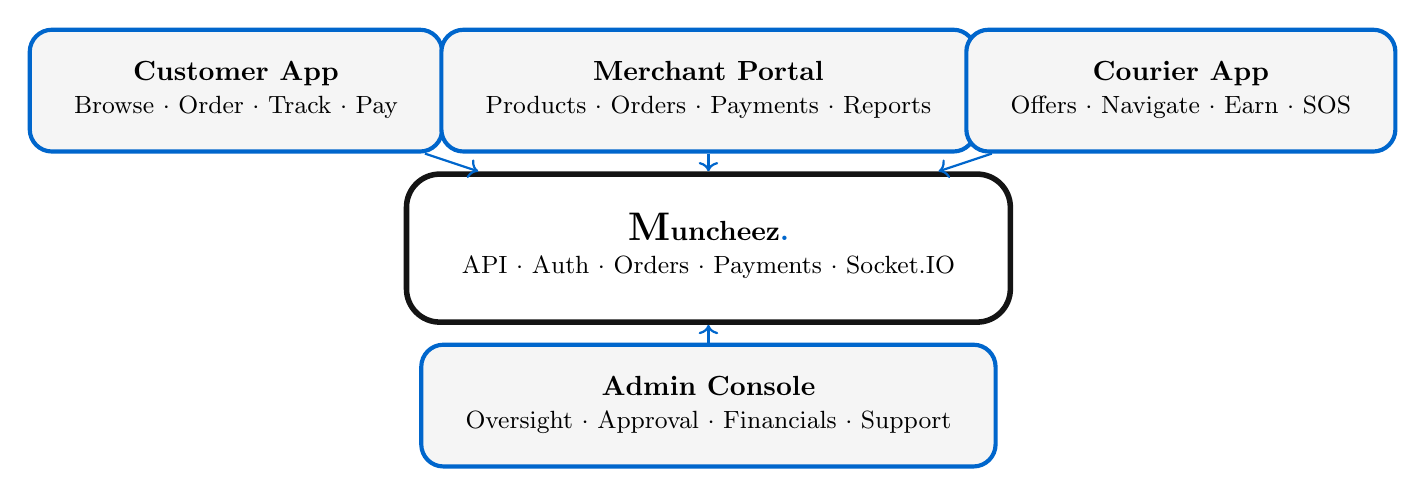
\begin{tikzpicture}
    % Customer
    \node[draw=MuncheezBlue, line width=1.5pt, rounded corners=8pt, fill=MuncheezLight, inner sep=10pt] (customer) at (-6,2) {
      \begin{tabular}{c}
        \textbf{Customer App}\\
        \small Browse $\cdot$ Order $\cdot$ Track $\cdot$ Pay
      \end{tabular}
    };
    
    % Merchant
    \node[draw=MuncheezBlue, line width=1.5pt, rounded corners=8pt, fill=MuncheezLight, inner sep=10pt] (merchant) at (0,2) {
      \begin{tabular}{c}
        \textbf{Merchant Portal}\\
        \small Products $\cdot$ Orders $\cdot$ Payments $\cdot$ Reports
      \end{tabular}
    };
    
    % Courier
    \node[draw=MuncheezBlue, line width=1.5pt, rounded corners=8pt, fill=MuncheezLight, inner sep=10pt] (courier) at (6,2) {
      \begin{tabular}{c}
        \textbf{Courier App}\\
        \small Offers $\cdot$ Navigate $\cdot$ Earn $\cdot$ SOS
      \end{tabular}
    };
    
    % Admin
    \node[draw=MuncheezBlue, line width=1.5pt, rounded corners=8pt, fill=MuncheezLight, inner sep=10pt] (admin) at (0,-2) {
      \begin{tabular}{c}
        \textbf{Admin Console}\\
        \small Oversight $\cdot$ Approval $\cdot$ Financials $\cdot$ Support
      \end{tabular}
    };
    
    % Core
    \node[draw=MuncheezDark, line width=2pt, rounded corners=12pt, fill=white, inner sep=14pt] (core) at (0,0) {
      \begin{tabular}{c}
        \textbf{\muncheezlogo}\\
        \small API $\cdot$ Auth $\cdot$ Orders $\cdot$ Payments $\cdot$ Socket.IO
      \end{tabular}
    };
    
    \draw[->, thick, MuncheezBlue] (customer) -- (core);
    \draw[->, thick, MuncheezBlue] (merchant) -- (core);
    \draw[->, thick, MuncheezBlue] (courier) -- (core);
    \draw[->, thick, MuncheezBlue] (admin) -- (core);
  \end{tikzpicture}
  
  \vspace{4mm}
  {\small\itshape Backend: Express + Prisma + Socket.IO \textbullet\ Frontend: React + Vite}
\end{frame}

% ═══════════════════════════════════════════════════════════════════════════
% SLIDE 10: THE MVP
% ═══════════════════════════════════════════════════════════════════════════
\begin{frame}{The MVP}
  \centering
  \vspace{4mm}
  
  
\begin{tikzpicture}
    \node[text width=0.9\textwidth, align=center] at (0,0) {
      {\Large\bfseries The initial product does not need to solve all of Kenya.}
    };
  \end{tikzpicture}
  
  \vspace{6mm}
  
  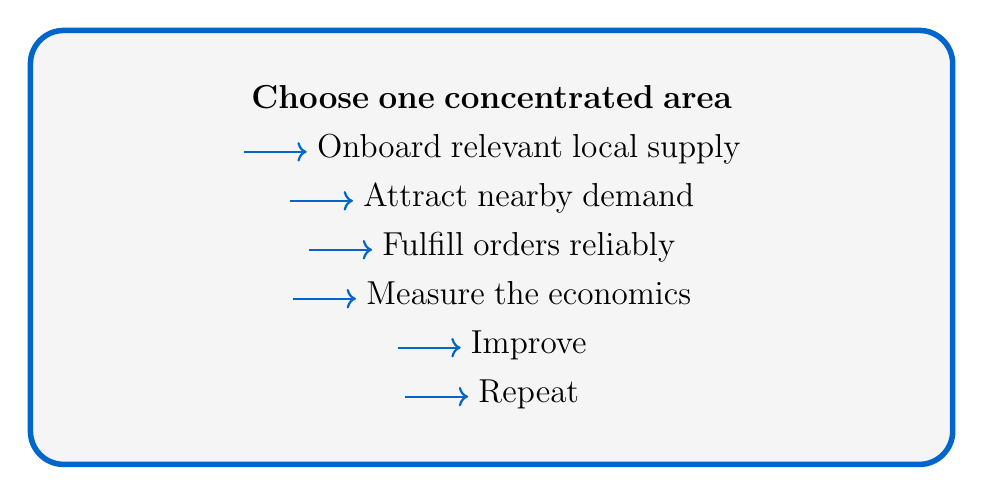
\begin{tikzpicture}
    \node[draw=MuncheezBlue, line width=2pt, rounded corners=12pt, fill=MuncheezLight, inner sep=20pt, text width=0.85\textwidth, align=center] {
      {\large\bfseries Choose one concentrated area}\\[2mm]
      \flowarrow\ {\large Onboard relevant local supply}\\[2mm]
      \flowarrow\ {\large Attract nearby demand}\\[2mm]
      \flowarrow\ {\large Fulfill orders reliably}\\[2mm]
      \flowarrow\ {\large Measure the economics}\\[2mm]
      \flowarrow\ {\large Improve}\\[2mm]
      \flowarrow\ {\large Repeat}
    };
  \end{tikzpicture}
  
  \vspace{6mm}
  
  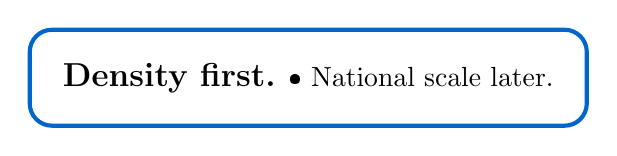
\begin{tikzpicture}
    \node[draw=MuncheezBlue, line width=1.5pt, rounded corners=8pt, fill=white, inner sep=12pt] {
      \textbf{\large Density first.} \textbullet\ National scale later.
    };
  \end{tikzpicture}
\end{frame}

% ═══════════════════════════════════════════════════════════════════════════
% SLIDE 11: BUSINESS MODEL
% ═══════════════════════════════════════════════════════════════════════════
\begin{frame}{Business Model}
  \begin{columns}[T]
    \begin{column}{0.48\textwidth}
      \sectiontitle{Revenue Streams}
      \vspace{3mm}
      \begin{itemize}
        \item \textbf{Merchant commission} \textbullet\ 15\% of order value
        \item \textbf{Customer delivery fees} \textbullet\ Per-order logistics charge
        \item \textbf{Future merchant services} \textbullet\ Marketing, analytics, premium tools
        \item \textbf{Promotional / advertising revenue} \textbullet\ Sponsored placements
        \item \textbf{Other services} \textbullet\ As marketplace grows
      \end{itemize}
    \end{column}
    \begin{column}{0.48\textwidth}
      \sectiontitle{Unit Economics}
      \vspace{3mm}
      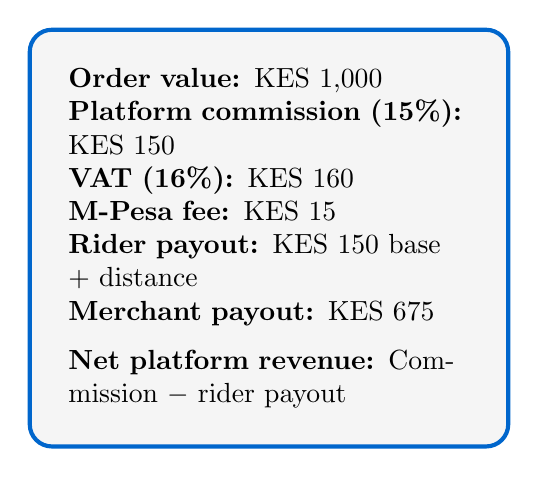
\begin{tikzpicture}
        \node[draw=MuncheezBlue, line width=1.5pt, rounded corners=8pt, fill=MuncheezLight, inner sep=14pt, text width=0.42\textwidth, align=left] {
          \textbf{Order value:} KES 1,000\\
          \textbf{Platform commission (15\%):} KES 150\\
          \textbf{VAT (16\%):} KES 160\\
          \textbf{M-Pesa fee:} KES 15\\
          \textbf{Rider payout:} KES 150 base + distance\\
          \textbf{Merchant payout:} KES 675\\
          \vspace{2mm}
          \textbf{Net platform revenue:} Commission $-$ rider payout
        };
      \end{tikzpicture}
      
      \vspace{6mm}
      
\begin{tikzpicture}
        \node[draw=MuncheezBlue, line width=2pt, rounded corners=12pt, fill=white, inner sep=12pt, text width=0.42\textwidth, align=center] {
          \textbf{\itshape Initial economics will be validated during the pilot.}
        };
      \end{tikzpicture}
    \end{column}
  \end{columns}
\end{frame}

% ═══════════════════════════════════════════════════════════════════════════
% SLIDE 12: COMPETITION
% ═══════════════════════════════════════════════════════════════════════════
\begin{frame}{Competition}
  \begin{columns}[T]
    \begin{column}{0.48\textwidth}
      \sectiontitle{Existing platforms}
      \vspace{3mm}
      Built strong delivery networks around established restaurants.
      
      \vspace{4mm}
      They serve supply that is already digitally capable.
    \end{column}
    \begin{column}{0.48\textwidth}
      \sectiontitle{Muncheez}
      \vspace{3mm}
      Starts from the other side of the market:
      
      \vspace{3mm}
      \begin{itemize}
        \item Fragmented local supply
        \item Underserved neighborhood demand
        \item Local logistics built from scratch
        \item Infrastructure around discovery, addressing, and delivery
      \end{itemize}
    \end{column}
  \end{columns}
  
  \vspace{6mm}
  \centering
  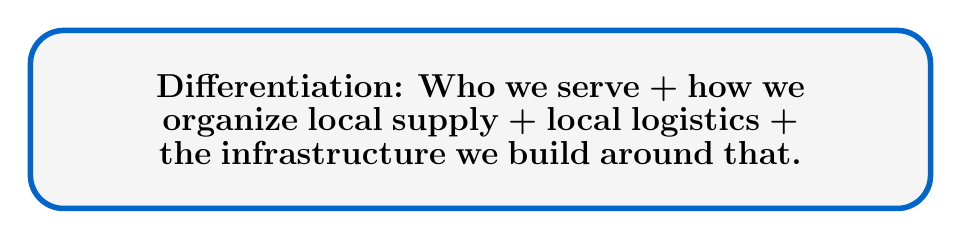
\begin{tikzpicture}
    \node[draw=MuncheezBlue, line width=2pt, rounded corners=12pt, fill=MuncheezLight, inner sep=16pt, text width=0.85\textwidth, align=center] {
      {\large\bfseries Differentiation: Who we serve + how we organize local supply + local logistics + the infrastructure we build around that.}
    };
  \end{tikzpicture}
\end{frame}

% ═══════════════════════════════════════════════════════════════════════════
% SLIDE 13: GO-TO-MARKET
% ═══════════════════════════════════════════════════════════════════════════
\begin{frame}{Go-to-Market}
  \centering
  \vspace{4mm}
  
  
\begin{tikzpicture}
    \node[text width=0.9\textwidth, align=center] at (0,0) {
      {\Large\bfseries Start in one concentrated area.}
    };
  \end{tikzpicture}
  
  \vspace{6mm}
  
  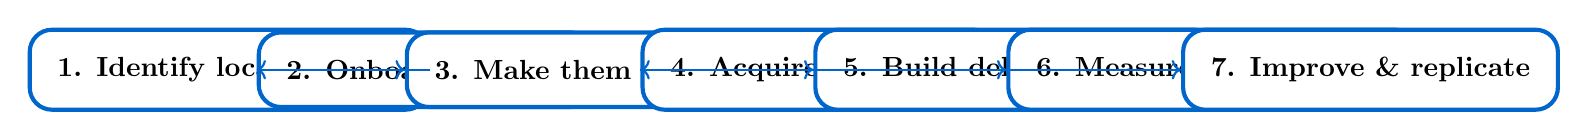
\begin{tikzpicture}
    \node[draw=MuncheezBlue, line width=1.5pt, rounded corners=8pt, fill=white, inner sep=10pt] (step1) at (-7,0) {\textbf{1. Identify local demand}};
    \node[draw=MuncheezBlue, line width=1.5pt, rounded corners=8pt, fill=white, inner sep=10pt] (step2) at (-4.5,0) {\textbf{2. Onboard vendors}};
    \node[draw=MuncheezBlue, line width=1.5pt, rounded corners=8pt, fill=white, inner sep=10pt] (step3) at (-2,0) {\textbf{3. Make them discoverable}};
    \node[draw=MuncheezBlue, line width=1.5pt, rounded corners=8pt, fill=white, inner sep=10pt] (step4) at (0.5,0) {\textbf{4. Acquire customers}};
    \node[draw=MuncheezBlue, line width=1.5pt, rounded corners=8pt, fill=white, inner sep=10pt] (step5) at (3,0) {\textbf{5. Build delivery density}};
    \node[draw=MuncheezBlue, line width=1.5pt, rounded corners=8pt, fill=white, inner sep=10pt] (step6) at (5.5,0) {\textbf{6. Measure repeat orders}};
    \node[draw=MuncheezBlue, line width=1.5pt, rounded corners=8pt, fill=white, inner sep=10pt] (step7) at (7.5,0) {\textbf{7. Improve \& replicate}};
    
    \draw[->, thick, MuncheezBlue] (step1) -- (step2);
    \draw[->, thick, MuncheezBlue] (step2) -- (step3);
    \draw[->, thick, MuncheezBlue] (step3) -- (step4);
    \draw[->, thick, MuncheezBlue] (step4) -- (step5);
    \draw[->, thick, MuncheezBlue] (step5) -- (step6);
    \draw[->, thick, MuncheezBlue] (step6) -- (step7);
  \end{tikzpicture}
  
  \vspace{6mm}
  {\small\itshape No unrealistic nationwide targets. Prove the model in one neighborhood, then expand.}
\end{frame}

% ═══════════════════════════════════════════════════════════════════════════
% SLIDE 14: WHAT SUCCESS MEANS
% ═══════════════════════════════════════════════════════════════════════════
\begin{frame}{What Success Means}
  \centering
  \vspace{4mm}
  
  {\Large\bfseries The first 6--12 months are about proving the model.}
  
  \vspace{6mm}
  
  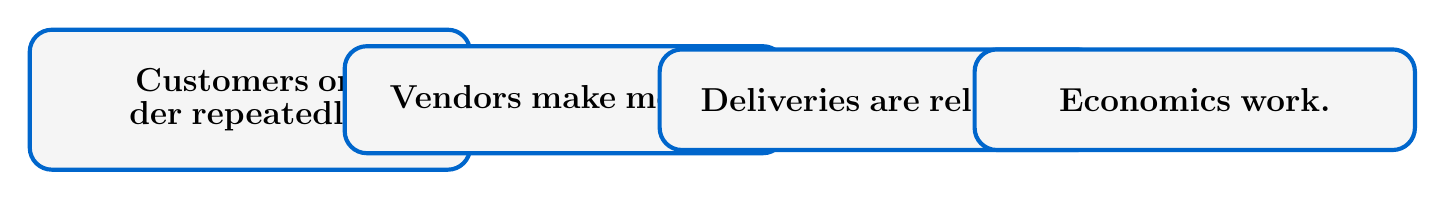
\begin{tikzpicture}
    \node[draw=MuncheezBlue, line width=1.5pt, rounded corners=8pt, fill=MuncheezLight, inner sep=14pt, text width=0.38\textwidth, align=center] (s1) at (-6,0) {
      \textbf{\large Customers order repeatedly.}
    };
    \node[draw=MuncheezBlue, line width=1.5pt, rounded corners=8pt, fill=MuncheezLight, inner sep=14pt, text width=0.38\textwidth, align=center] (s2) at (-2,0) {
      \textbf{\large Vendors make money.}
    };
    \node[draw=MuncheezBlue, line width=1.5pt, rounded corners=8pt, fill=MuncheezLight, inner sep=14pt, text width=0.38\textwidth, align=center] (s3) at (2,0) {
      \textbf{\large Deliveries are reliable.}
    };
    \node[draw=MuncheezBlue, line width=1.5pt, rounded corners=8pt, fill=MuncheezLight, inner sep=14pt, text width=0.38\textwidth, align=center] (s4) at (6,0) {
      \textbf{\large Economics work.}
    };
  \end{tikzpicture}
  
  \vspace{4mm}
  
  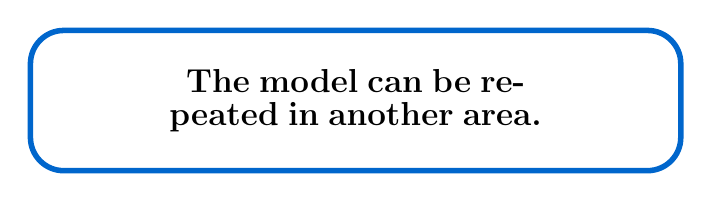
\begin{tikzpicture}
    \node[draw=MuncheezBlue, line width=2pt, rounded corners=12pt, fill=white, inner sep=14pt, text width=0.6\textwidth, align=center] at (0,-2.5) {
      \textbf{\large The model can be repeated in another area.}
    };
  \end{tikzpicture}
  
  \vspace{4mm}
  {\small\itshape More important than download counts or vendor numbers.}
\end{frame}

% ═══════════════════════════════════════════════════════════════════════════
% SLIDE 15: FUNDRAISING
% ═══════════════════════════════════════════════════════════════════════════
\begin{frame}{Fundraising}
  \centering
  \vspace{4mm}
  
  
\begin{tikzpicture}
    \node[text width=0.9\textwidth, align=center] at (0,1.5) {
      {\Huge\bfseries KES 15 Million}\\[2mm]
      {\large Pre-Seed Round}
    };
  \end{tikzpicture}
  
  \vspace{6mm}
  
  
\begin{tikzpicture}
    \node[draw=MuncheezBlue, line width=1.5pt, rounded corners=8pt, fill=MuncheezLight, inner sep=14pt, text width=0.85\textwidth, align=center] at (0,0) {
      \textbf{Capital to move from product development into real-world validation and launch.}
    };
  \end{tikzpicture}
  
  \vspace{6mm}
  
  \begin{columns}[T]
    \begin{column}{0.48\textwidth}
      \sectiontitle{What the money achieves}
      \vspace{3mm}
      \begin{itemize}
        \item Backend and infrastructure
        \item Maps and location infrastructure
        \item Payments integration
        \item Product completion
        \item Merchant onboarding
        \item Customer acquisition
      \end{itemize}
    \end{column}
    \begin{column}{0.48\textwidth}
      \sectiontitle{Operational requirements}
      \vspace{3mm}
      \begin{itemize}
        \item Delivery operations
        \item Team and operations
        \item Compliance
        \item Pilot market execution
        \item Repeatability validation
      \end{itemize}
    \end{column}
  \end{columns}
  
  \vspace{4mm}
  {\small\itshape Milestones and outcomes, not simply expenses.}
\end{frame}

% ═══════════════════════════════════════════════════════════════════════════
% SLIDE 16: THANK YOU / QUESTIONS
% ═══════════════════════════════════════════════════════════════════════════
\begin{frame}[plain]
  \centering
  \vfill
  
\begin{tikzpicture}
    \node[text width=0.9\textwidth, align=center] at (0,0) {
      {\fontsize{48}{52}\selectfont\textbf{\muncheezlogo}}\\[8mm]
      {\Large Thank you.}\\[4mm]
      {\large Questions?}\\[8mm]
      {\normalsize\itshape Local commerce, delivered.}
    };
  \end{tikzpicture}
  \vfill
\end{frame}

\end{document}
